\documentclass{beamer}

\usecolortheme[light]{solarized}

\beamertemplatenavigationsymbolsempty


\usepackage{booktabs}
\usepackage{graphicx}
\usepackage{hyperref}
\usepackage{minted}
\usepackage{moresize}
\usepackage{standalone}
\usepackage{tcolorbox}
\usepackage{tikz}
\usepackage[normalem]{ulem}
\usepackage{xpatch}
\usepackage{fix-cm}
\usepackage{subcaption}

\xpatchcmd{\sout}
  {\bgroup}
    {\bgroup\def\ULthickness{2pt}}
      {}{}

\usetikzlibrary{calc, patterns}

\definecolor{twitter}{RGB}{64, 153, 255}
\definecolor{github}{RGB}{211, 211, 211}

\newcommand{\assetsfolder}{./assets}
\newcommand{\revisitresearchfolder}{$HOME/rsc/revisiting-axelrod-second}
\newcommand{\moranresearchfolder}{$HOME/rsc/axelrod-moran}
\newcommand{\mlresearchfolder}{$HOME/rsc/ml-paper}

\begin{document}

    \begin{frame}
        \begin{center}
            \Huge
                Reflecting on a transitive Summer School in Namibia

               \vfill

            \Large
               Rob Wilson\\
               Vince Knight \href{https://twitter.com/drvinceknight}{@drvinceknight}\\
               Many more
        \end{center}

    \end{frame}

    \begin{frame}
        \begin{center}
            \Large
            \url{www.cardiff.ac.uk/phoenix-project}
        \end{center}
    \end{frame}

    \begin{frame}
        \begin{center}
            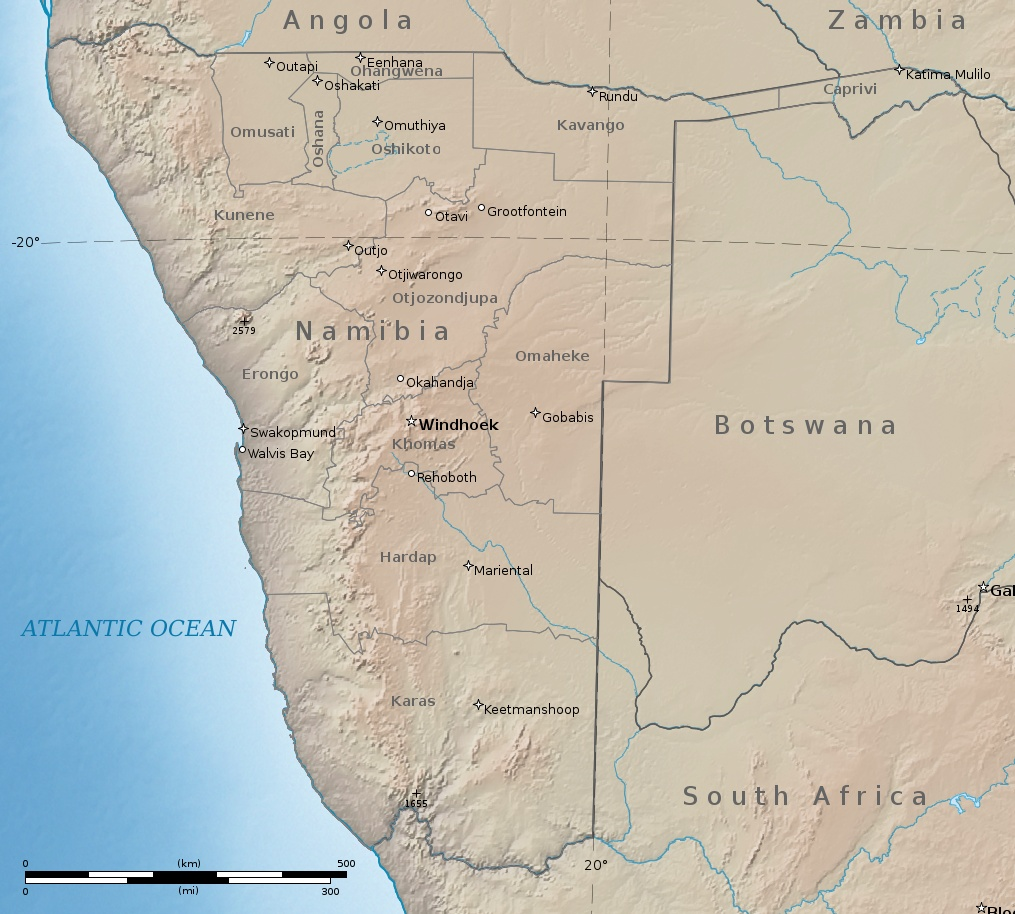
\includegraphics[width=.8\textwidth]{./assets/map_of_namibia.jpg}
        \end{center}
    \end{frame}

    \begin{frame}

        \begin{center}
            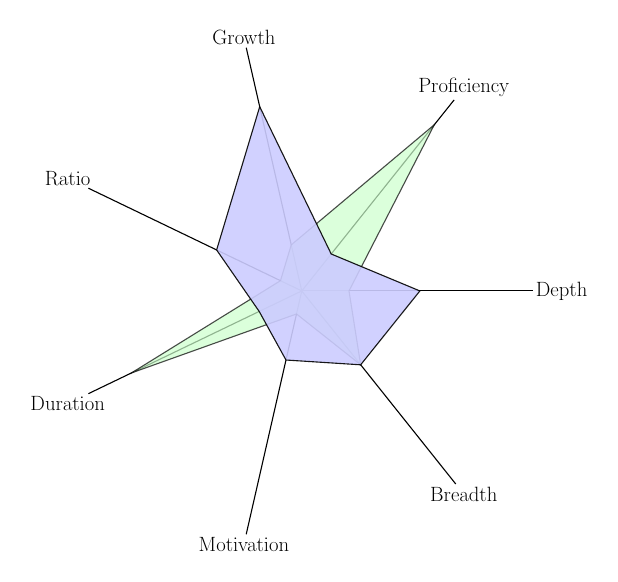
\begin{tikzpicture}[scale=0.3, every node/.style={scale=0.3}]
                \coordinate (origin) at (0, 0);

                \foreach[count=\i] \radius/\dim in {9/Proficiency,
                                                    2/Growth,
                                                    1/Ratio,
                                                    8/Duration,
                                                    1/Motivation,
                                                    4/Breadth,
                                                    2/Depth}{
                    \coordinate (\i) at (\i * 360 / 7: \radius);
                    \node (title) at (\i * 360 / 7: 11) {\Huge\dim};
                    \draw (origin) -- (title);
                }

                \draw [fill=green!20, opacity=.7] (1)
                                            \foreach \i in {2,...,7}{-- (\i)} --cycle;

                \pause

                \foreach[count=\i] \radius/\dim in {2/Proficiency,
                                                    8/Growth,
                                                    4/Ratio,
                                                    2/Duration,
                                                    3/Motivation,
                                                    4/Breadth,
                                                    5/Depth}{
                    \coordinate (\i) at (\i * 360 / 7: \radius);
                    \node (title) at (\i * 360 / 7: 11) {};
                }

                \draw [fill=blue!20, opacity=.9] (1)
                                            \foreach \i in {2,...,7}{-- (\i)} --cycle;
            \end{tikzpicture}
        \end{center}
    \end{frame}

    \begin{frame}
        \Large
        \begin{center}
            \begin{itemize}
                \setlength\itemsep{1em}
                \item Morning \& afternoon workshops over 2 weeks
                \item Sessions based on mathematical topics
                \item Three groups of ~20 students
                \item Aim to encourage exploration and develop confidence
            \end{itemize}
        \end{center}
    \end{frame}

    \begin{frame}
        \begin{center}
            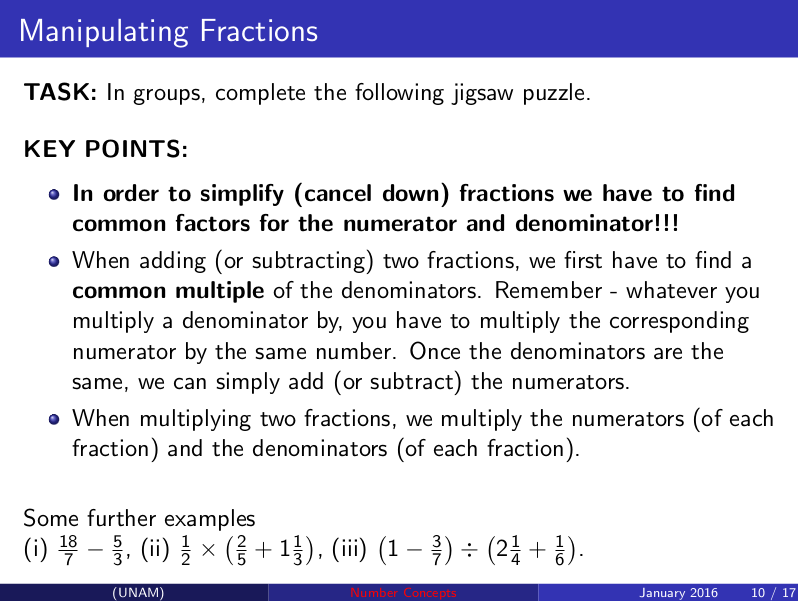
\includegraphics[width=.3\textwidth]{./assets/example_resources_2015.png}
            \hspace{.1cm}
            \framebox{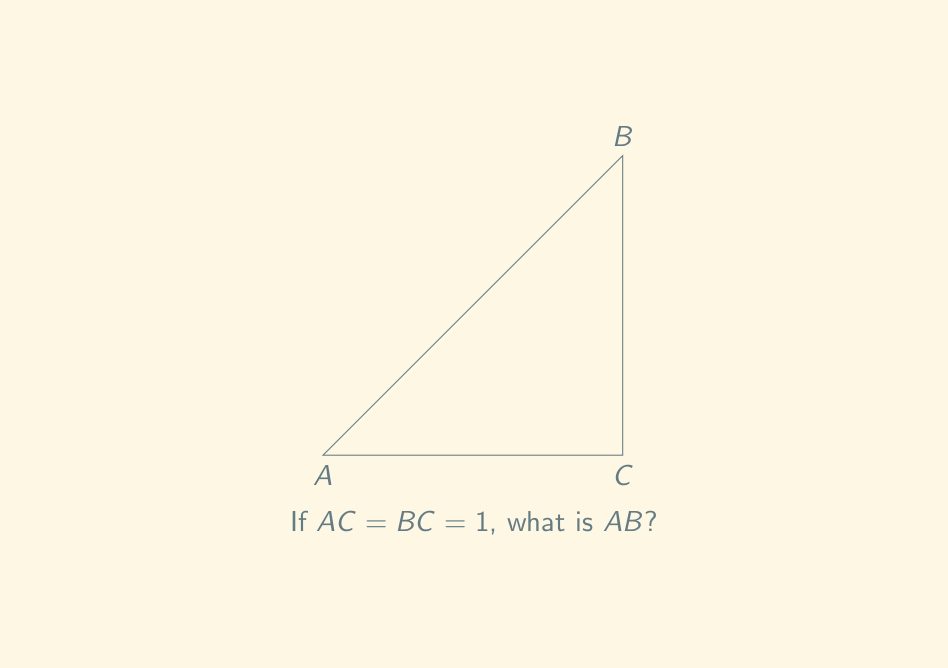
\includegraphics[width=.3\textwidth]{./assets/example_resources_2016.png}}
            \hspace{.1cm}
            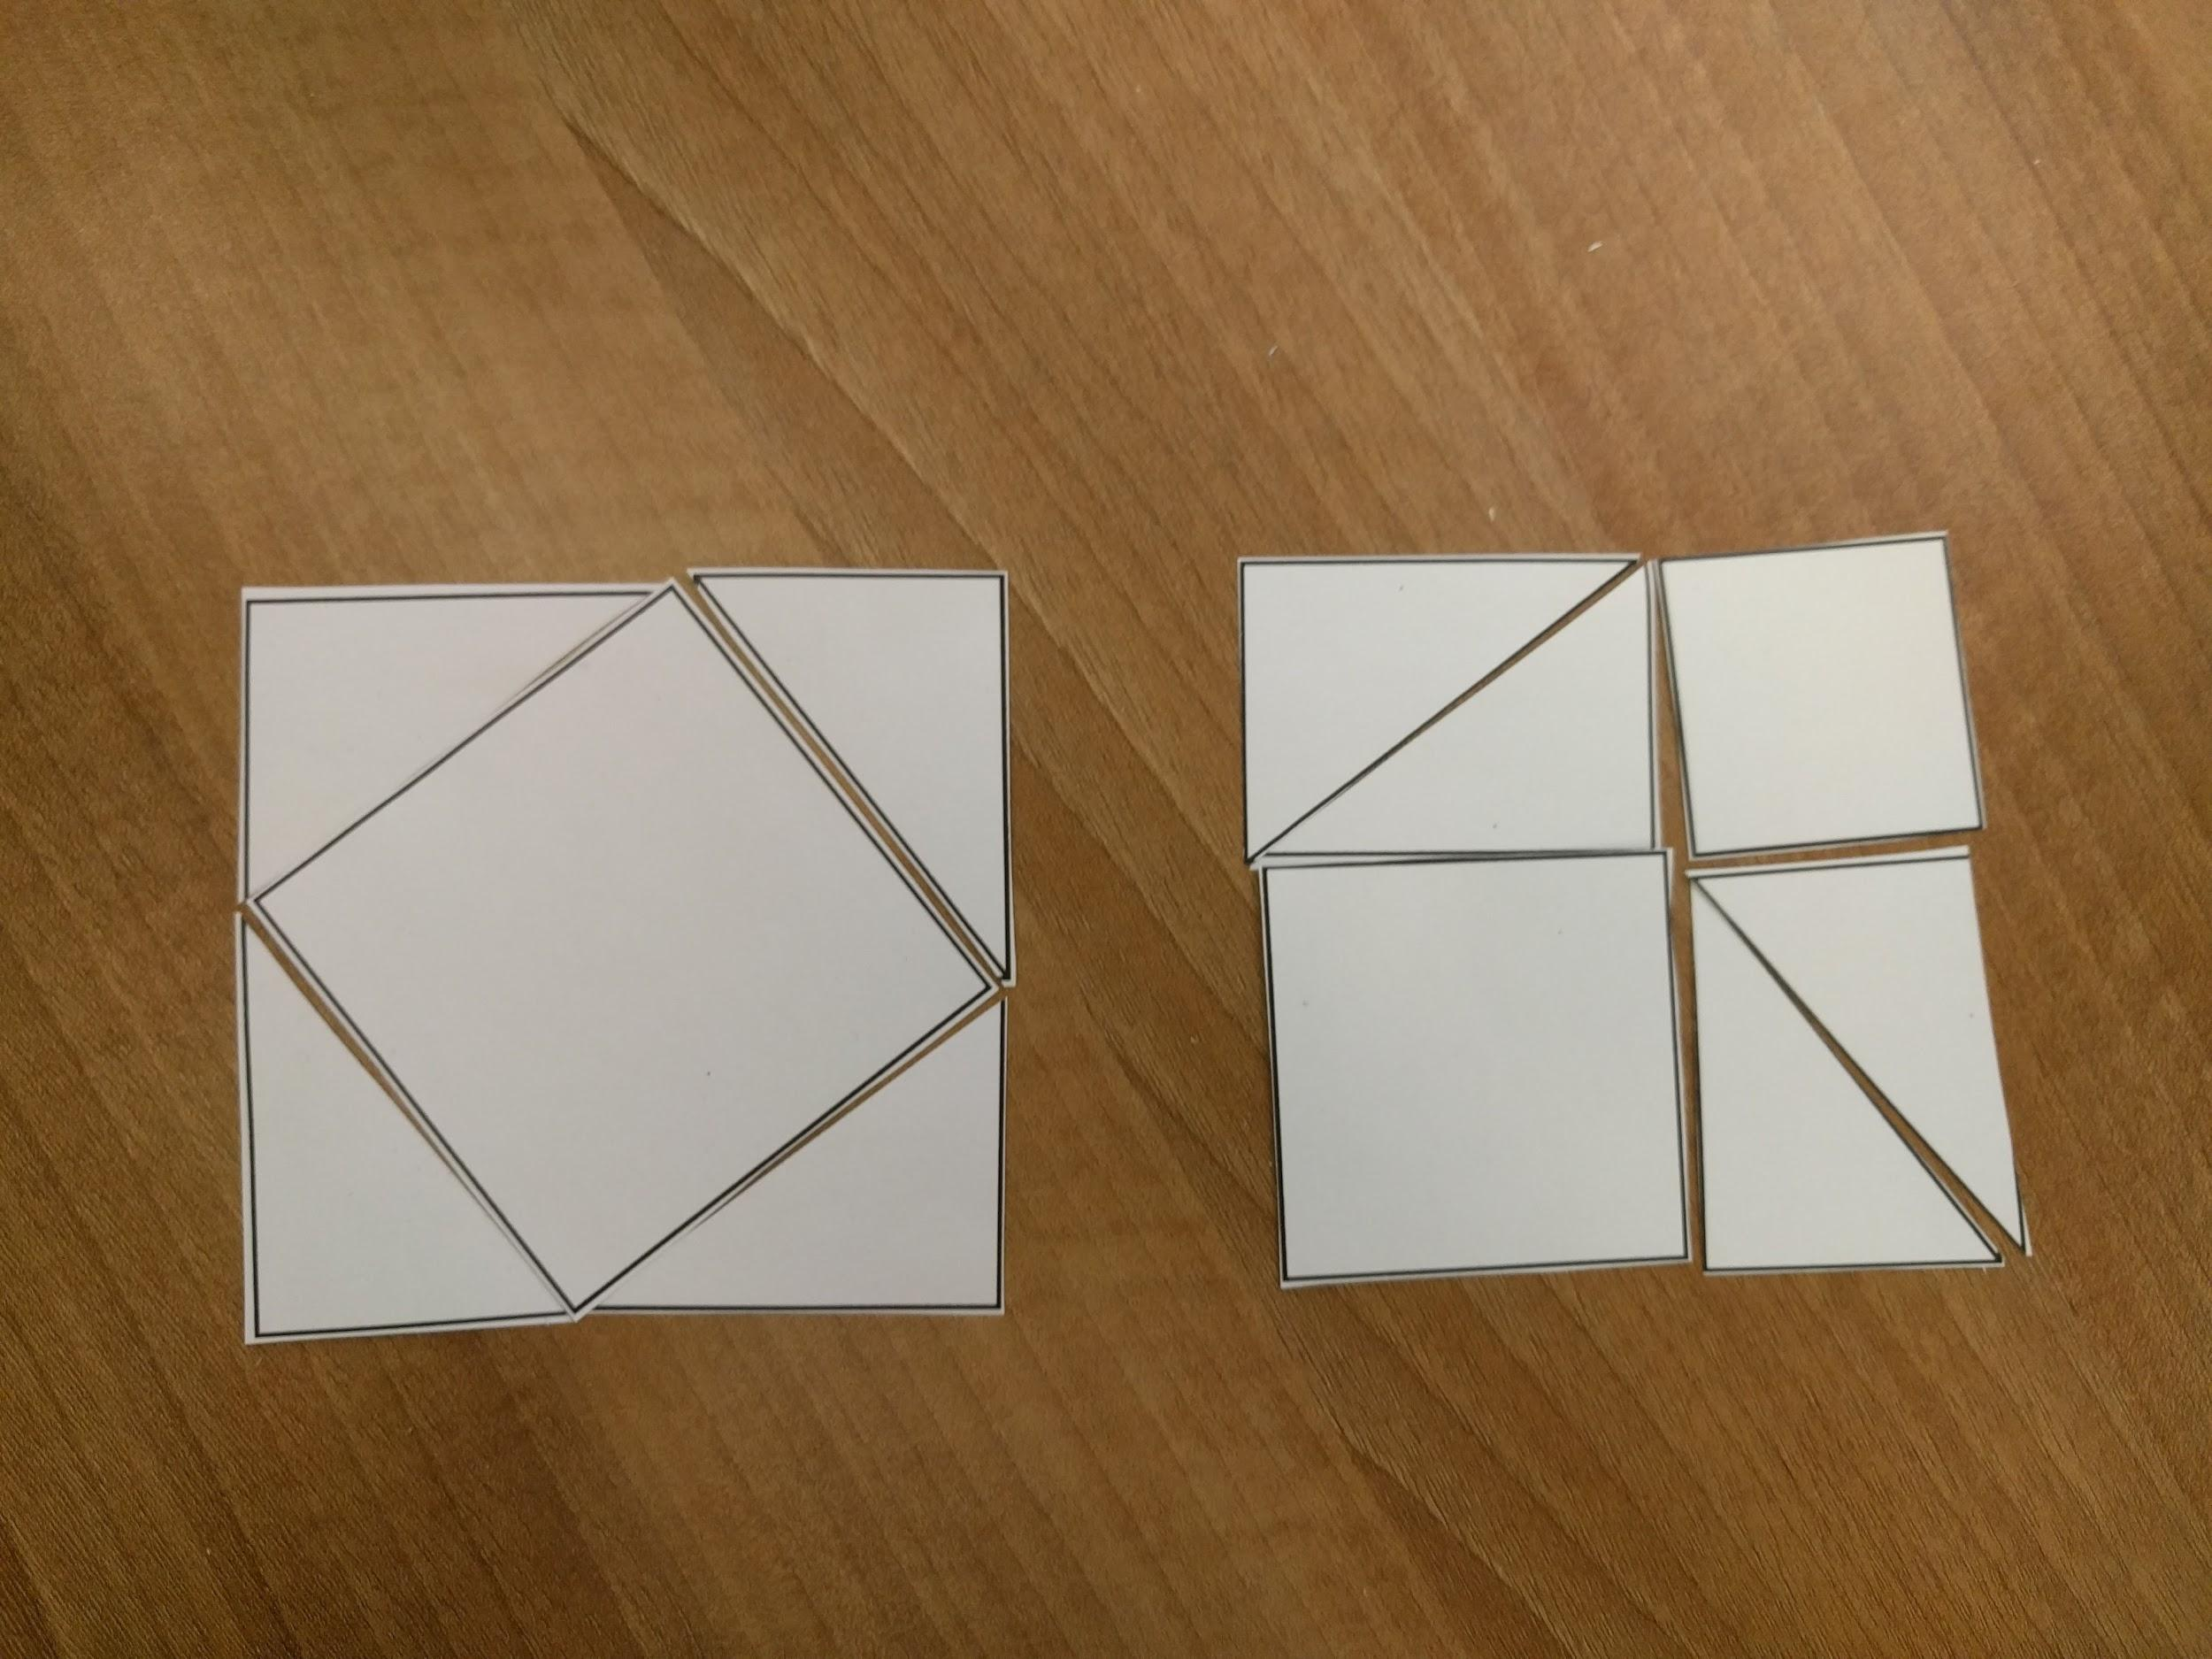
\includegraphics[width=.3\textwidth]{./assets/example_resources_2017.png}

            \vfill
            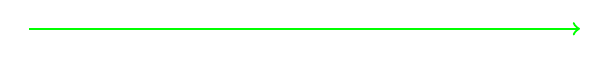
\begin{tikzpicture}
                \draw [green, thick, ->] (3, 0) -- (10, 0);
            \end{tikzpicture}
        \end{center}

    \end{frame}

    \begin{frame}
        \begin{center}
            \begin{tikzpicture}
                \node (img1)
                    {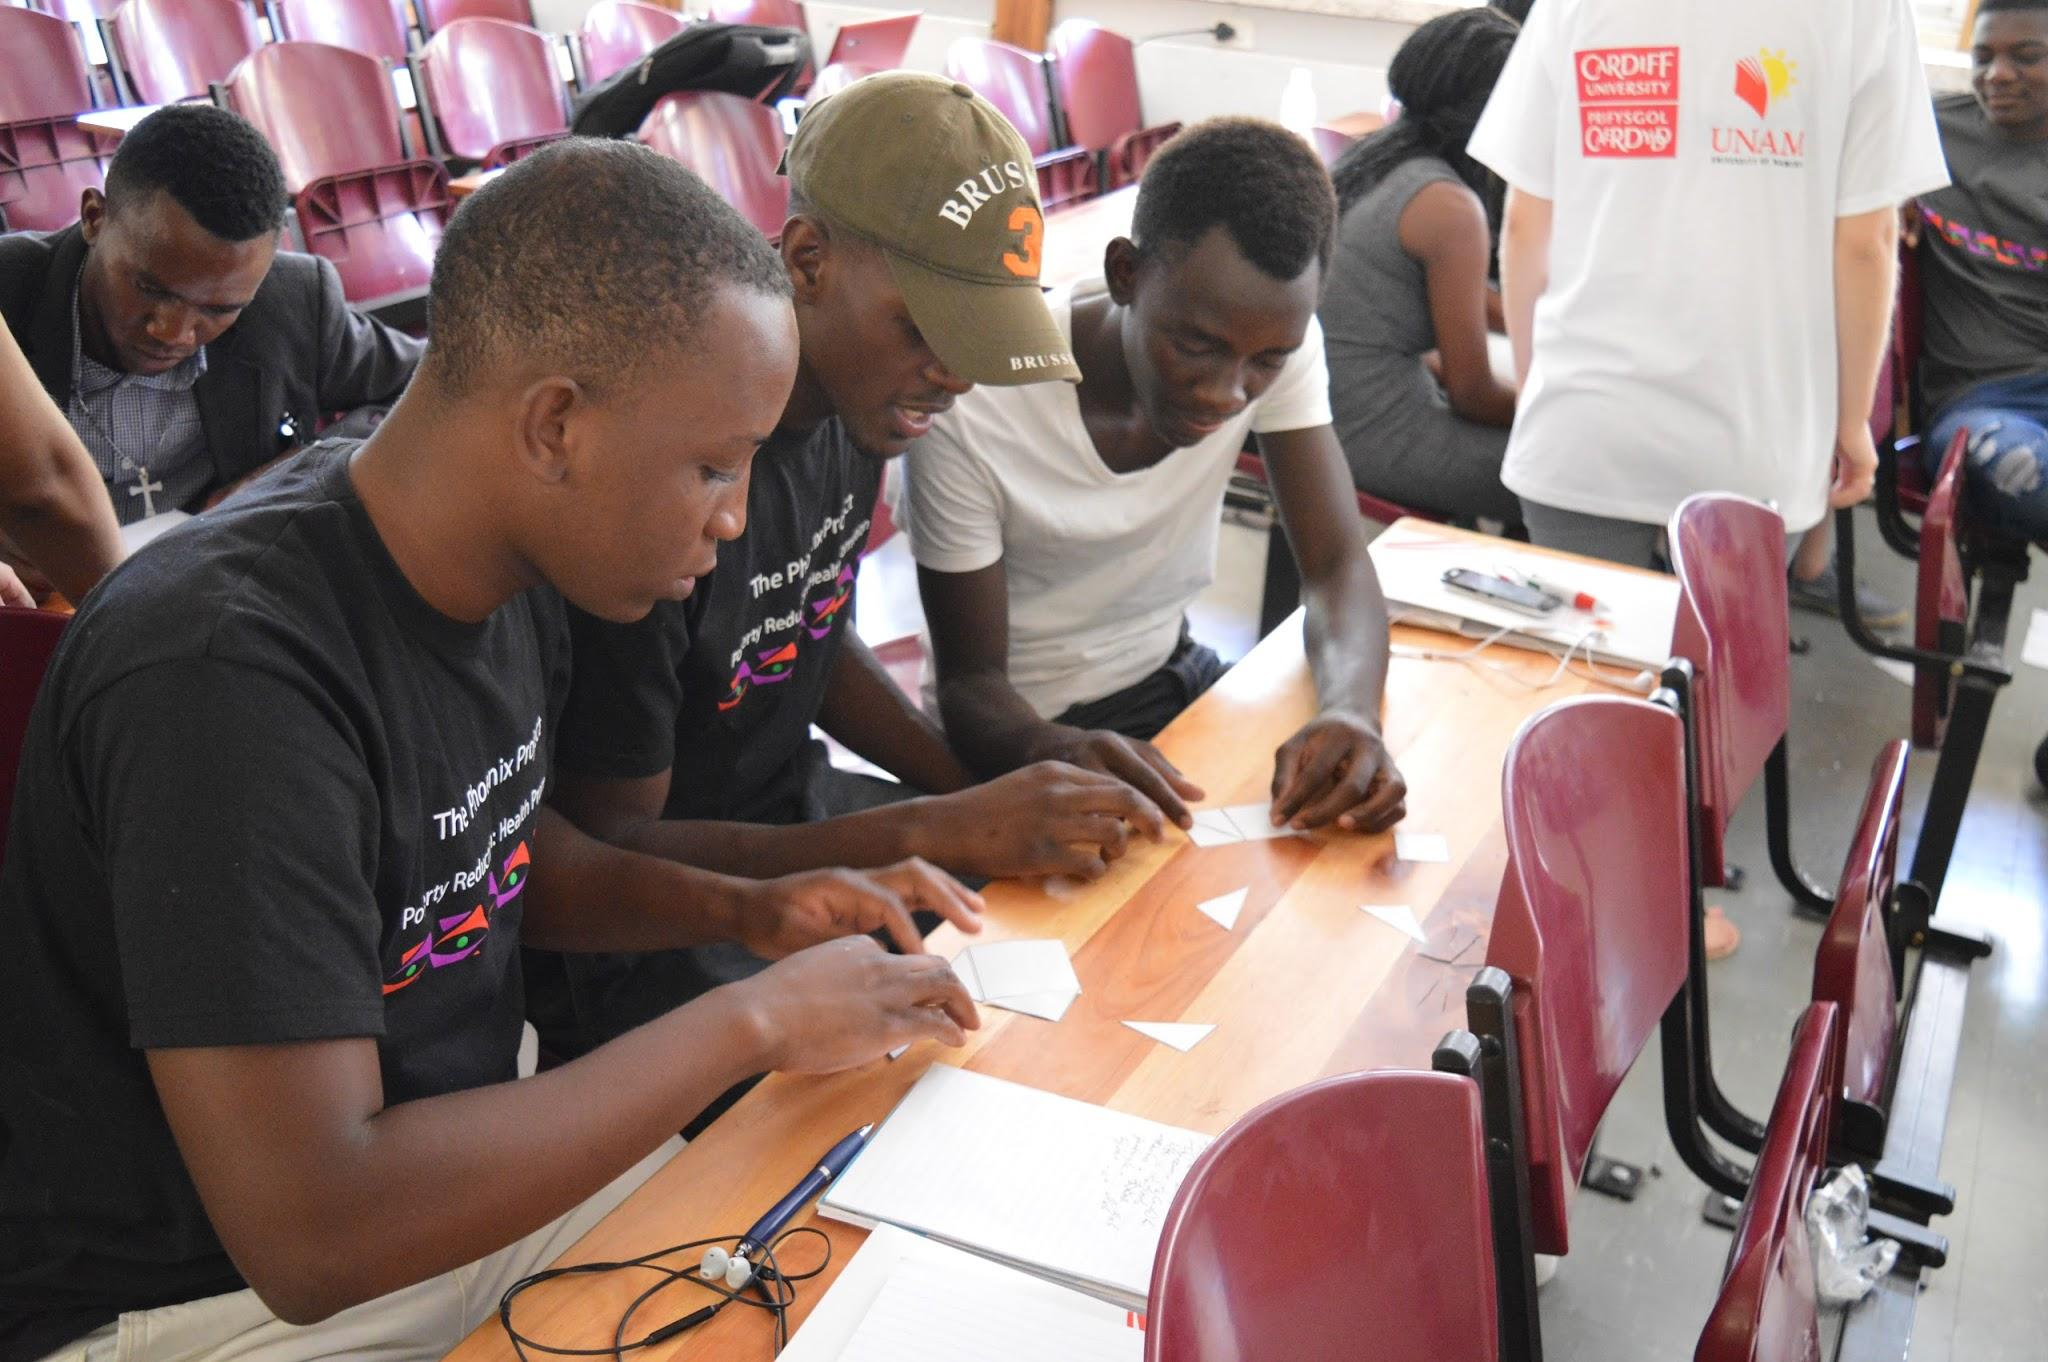
\includegraphics[width=.6\textwidth]{./assets/working_together_1.jpg}};
                \node (img2) at (img1.south east) [xshift=1cm]
                    {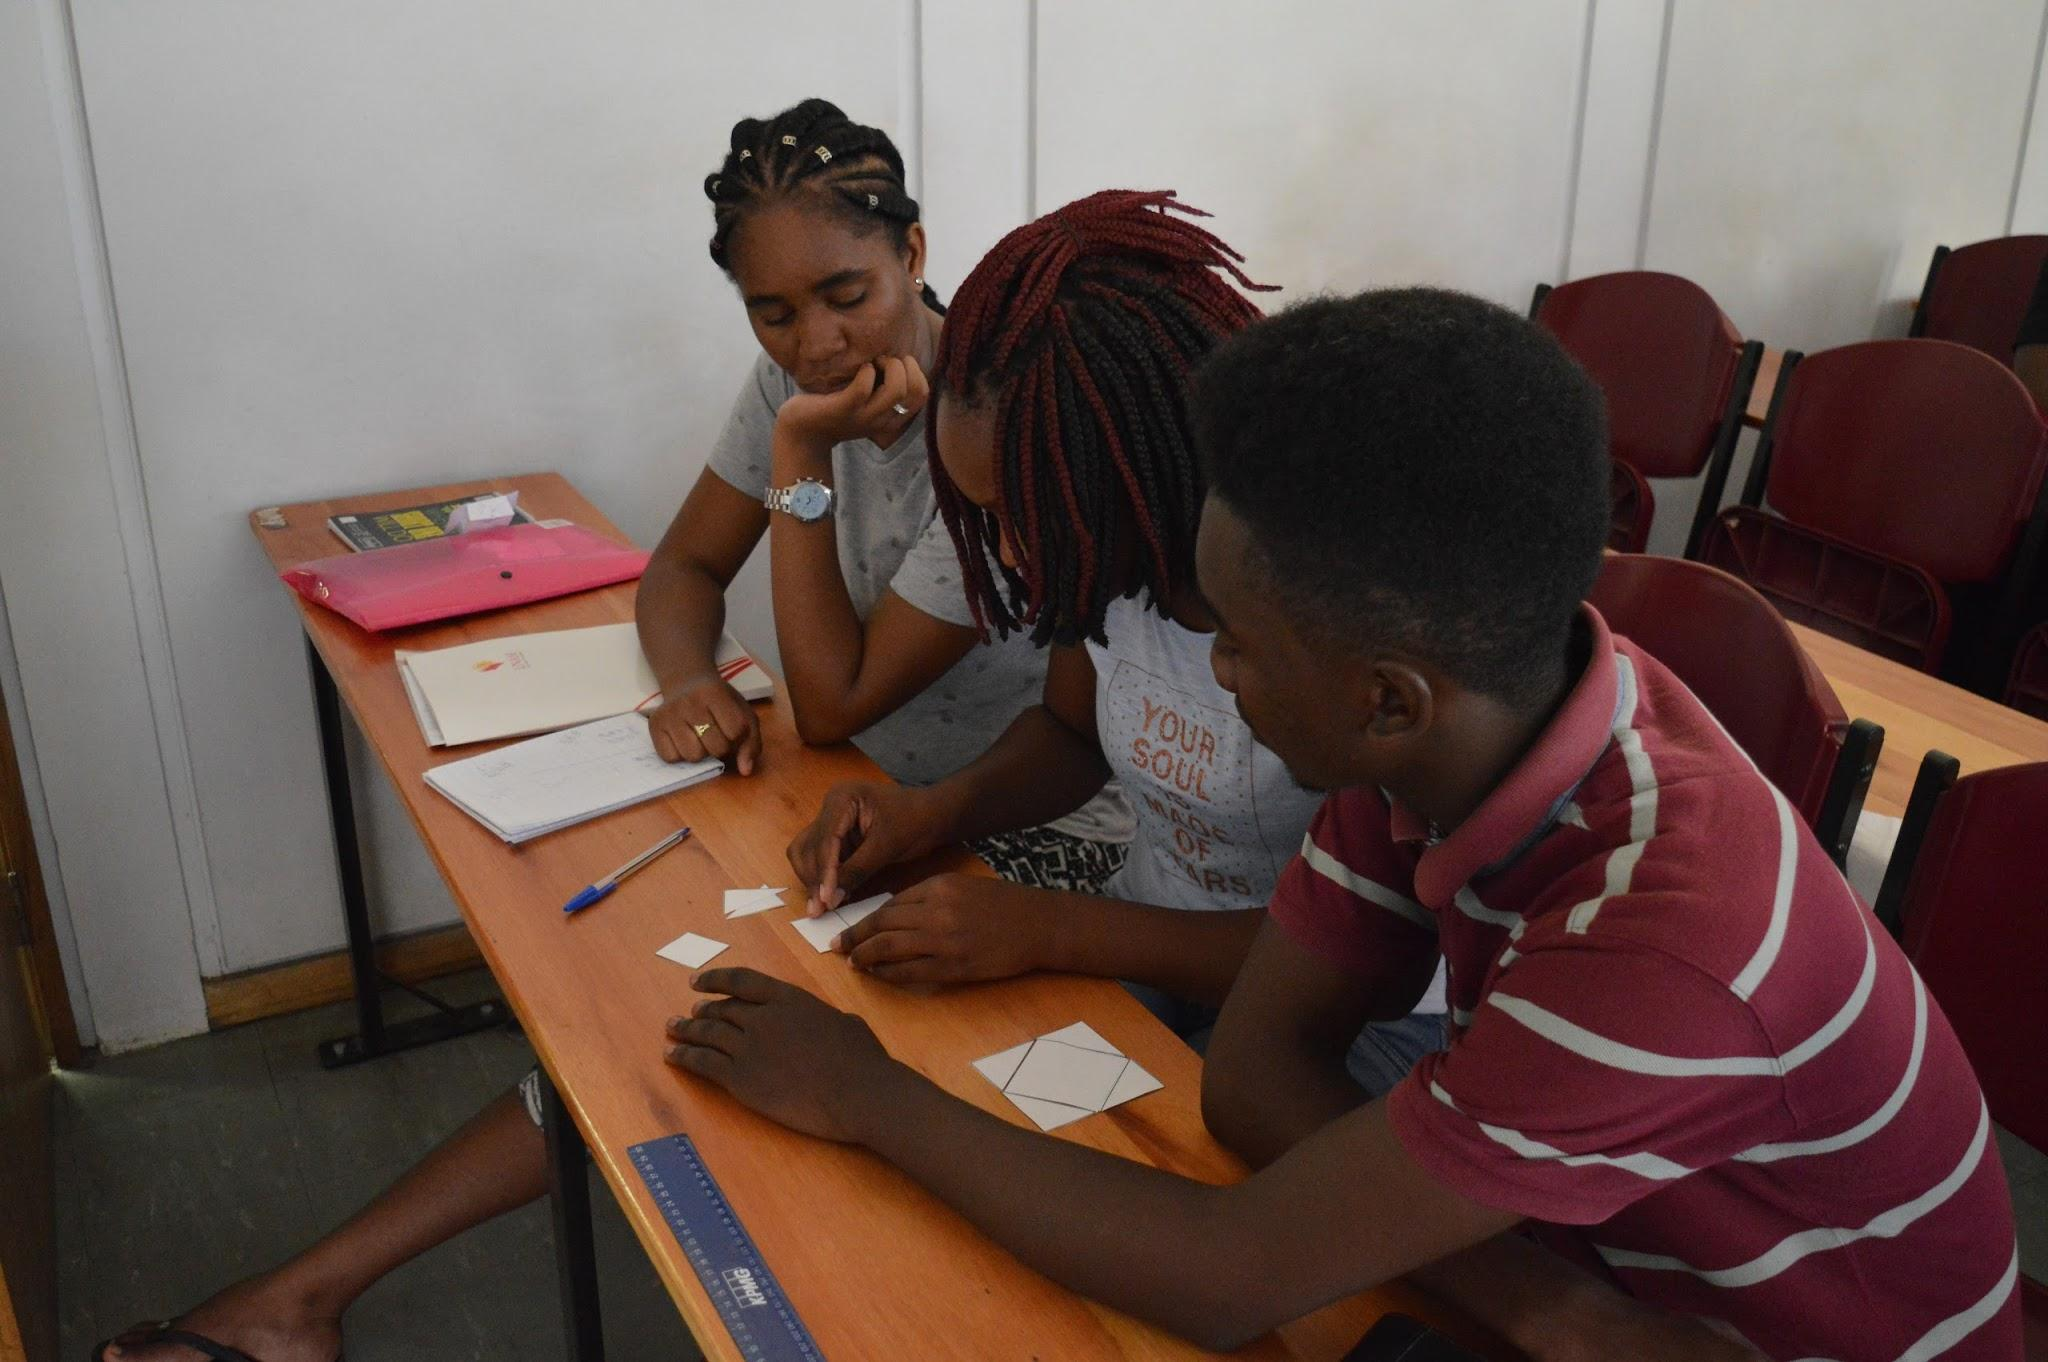
\includegraphics[width=.6\textwidth]{./assets/working_together_2.jpg}};
            \end{tikzpicture}
        \end{center}
    \end{frame}

    \begin{frame}
        \begin{center}
            \begin{tikzpicture}
                \node (img1)
                    {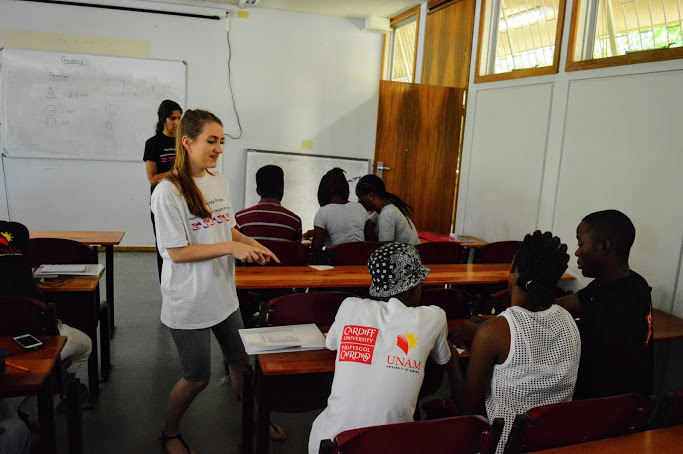
\includegraphics[width=.6\textwidth]{./assets/student_lead_1.png}};
                \node (img2) at (img1.north east) [xshift=1cm, yshift=1cm]
                    {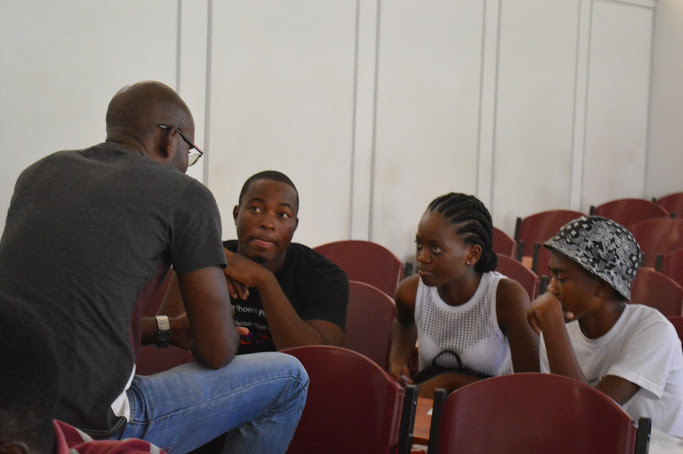
\includegraphics[width=.6\textwidth]{./assets/student_lead_2.png}};
            \end{tikzpicture}
        \end{center}
    \end{frame}

    \begin{frame}
        \begin{center}
            \begin{tikzpicture}
                \node (img1)
                    {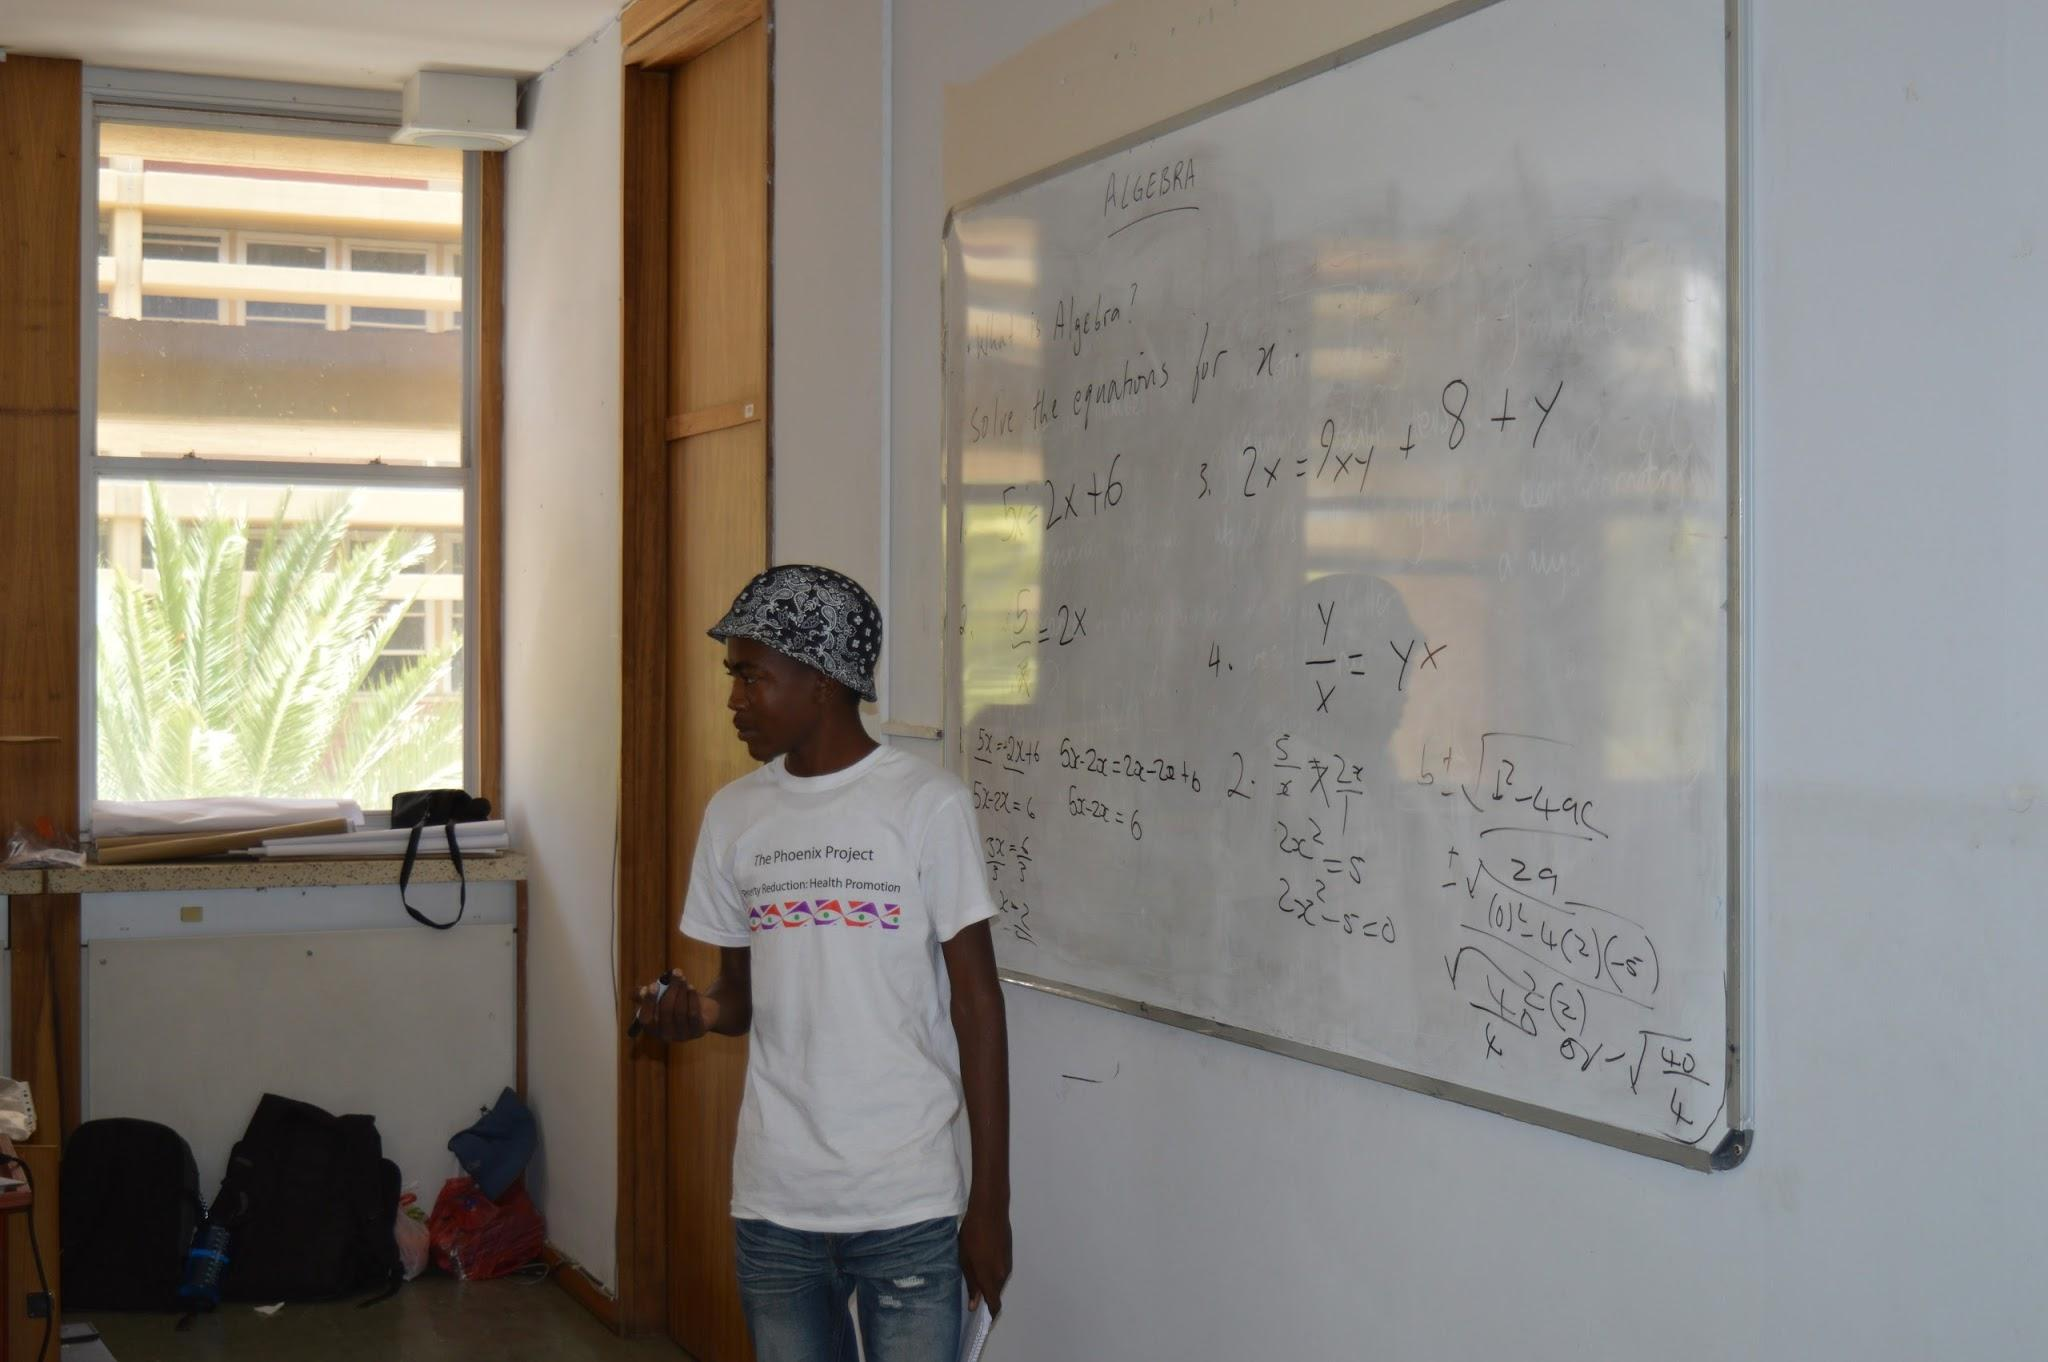
\includegraphics[width=.5\textwidth]{./assets/student_presentation_1.jpg}};
                \node (img2) at (img1.east) [xshift=3cm]
                    {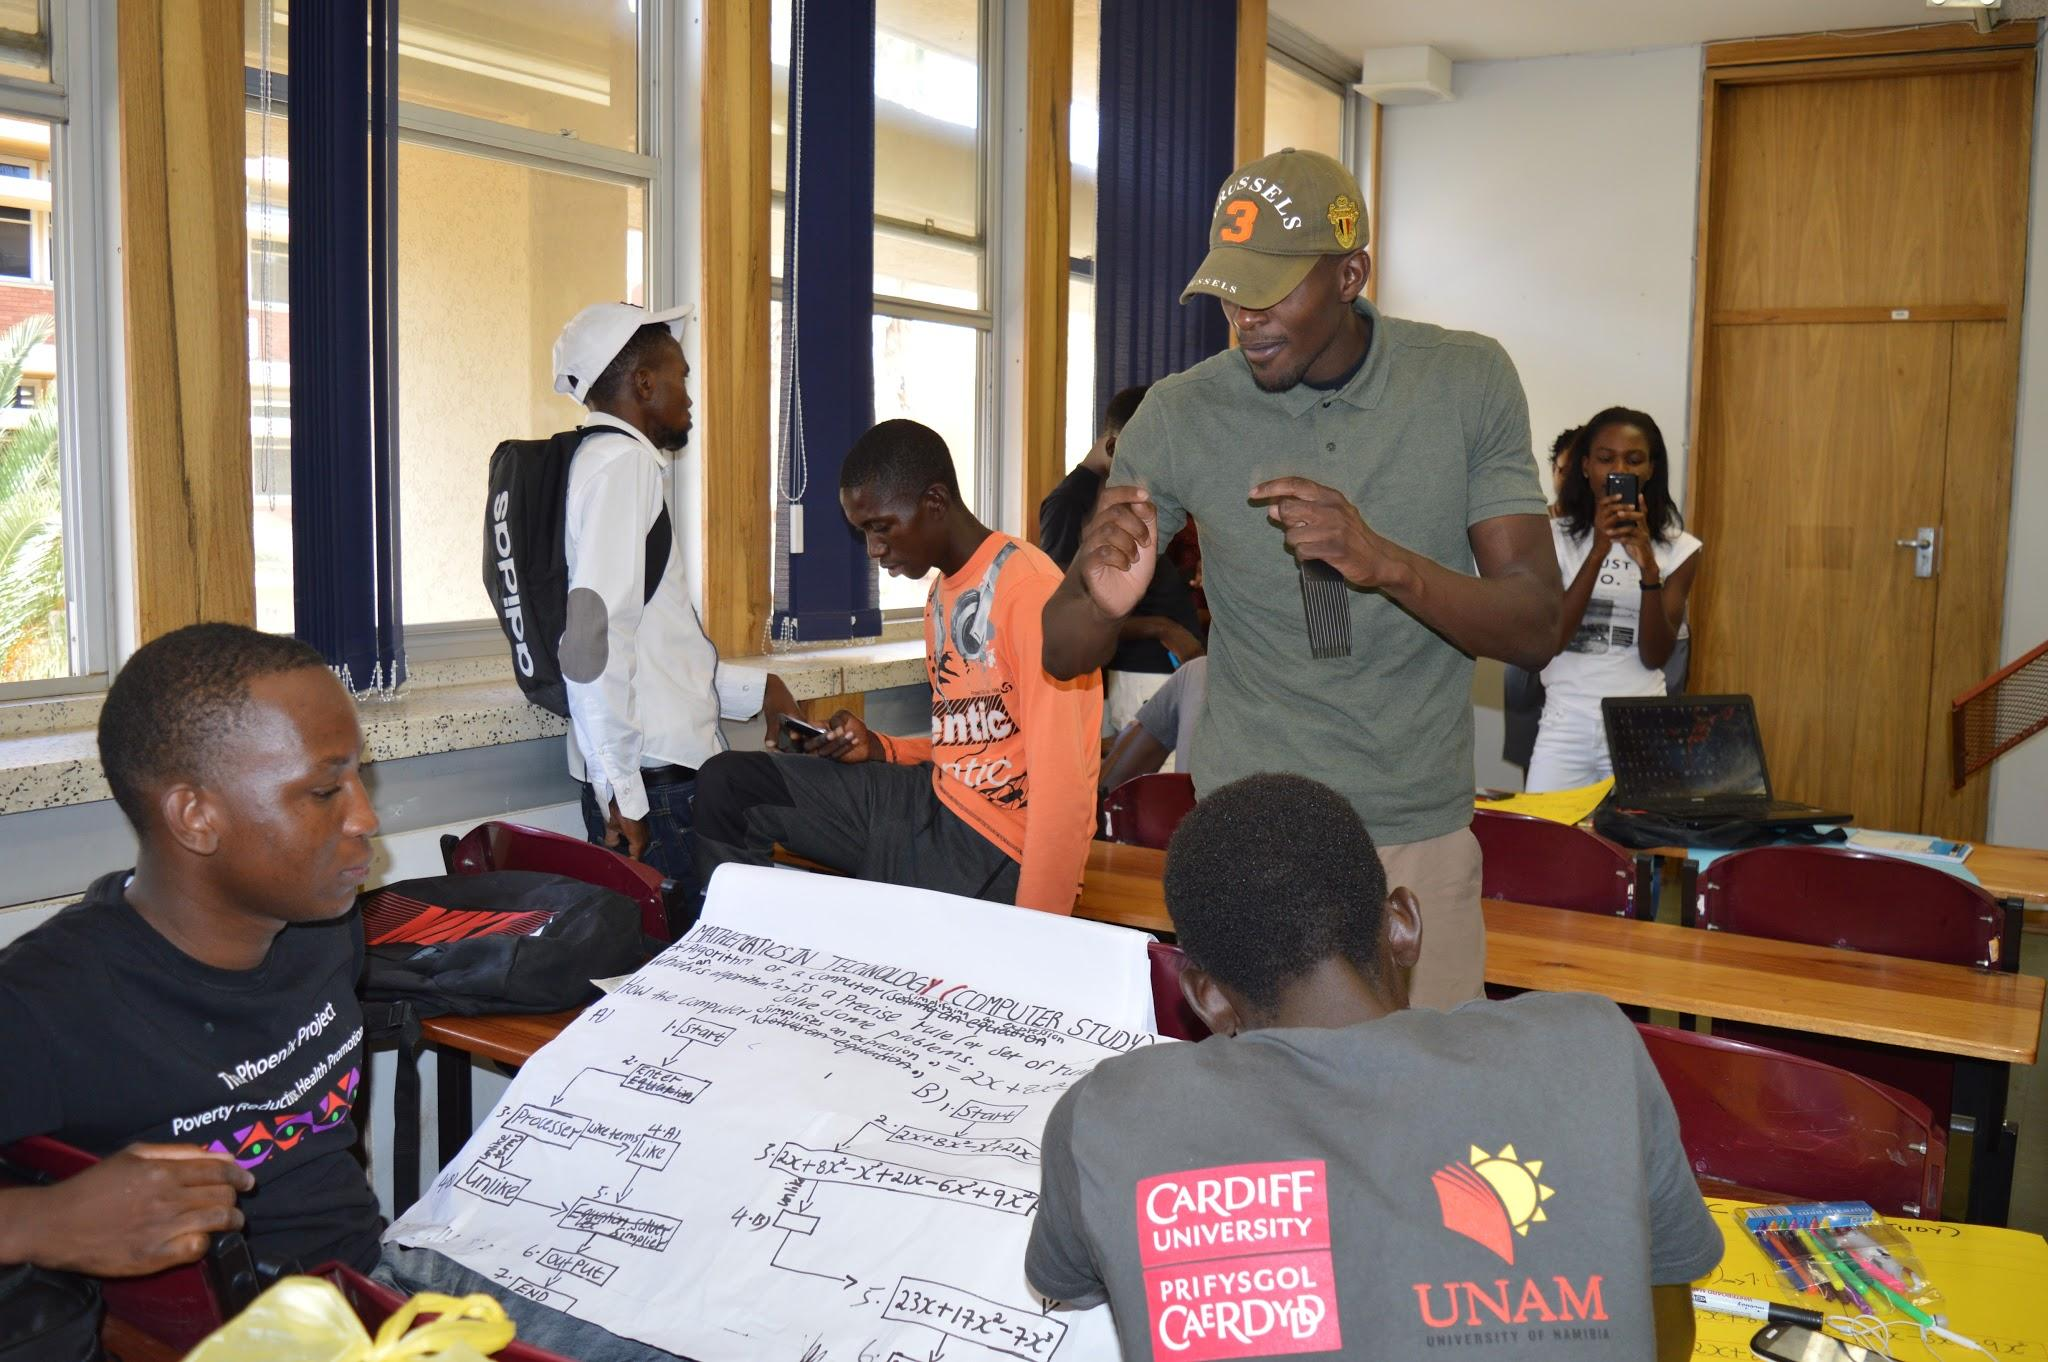
\includegraphics[width=.5\textwidth]{./assets/student_presentation_2.jpg}};
                \node (img3) at (img1.south east) [yshift=-2cm]
                    {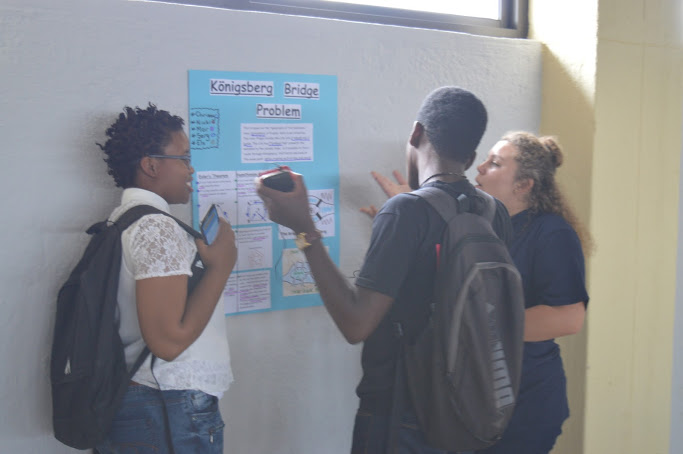
\includegraphics[width=.5\textwidth]{./assets/student_presentation_3.jpg}};
            \end{tikzpicture}
        \end{center}
    \end{frame}

    \begin{frame}
        \begin{center}
            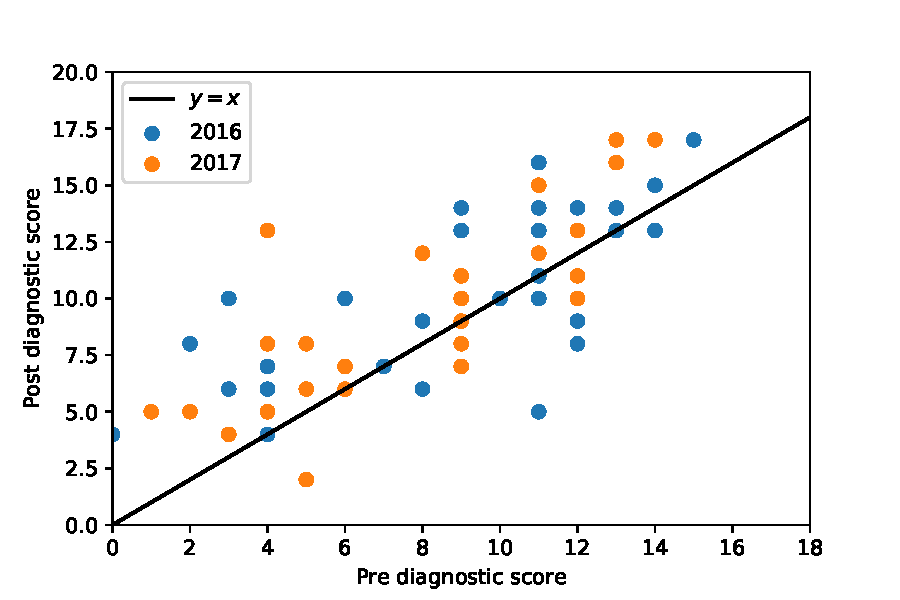
\includegraphics[width=.9\textwidth]{./assets/diagnostic_scores.pdf}
        \end{center}
    \end{frame}

    \begin{frame}
        \begin{table}[!hbtp]
            \tiny
            \centering

            \begin{subfigure}[t]{.5\textwidth}
                \centering
                \begin{tabular}{lrrr}
\toprule
           Dimension &    5\% &  Median &   95\% \\
\midrule
        Extraversion &  0.24 &    0.50 &  0.88 \\
        Agreableness &  0.04 &    0.40 &  0.76 \\
   Conscientiousness &  0.29 &    0.71 &  1.00 \\
 Emotional Stability &  0.04 &    0.27 &  0.55 \\
            Openness &  0.30 &    0.75 &  1.00 \\
            Strength &  0.14 &    0.27 &  0.96 \\
          Confidence &  0.20 &    0.42 &  1.00 \\
\bottomrule
\end{tabular}

                \caption{Above
                median}
            \end{subfigure}%
            ~
            \begin{subfigure}[t]{.5\textwidth}
                \centering
                \begin{tabular}{lrrr}
\toprule
           Dimension &    5\% &  Median &   95\% \\
\midrule
        Extraversion &  0.10 &    0.50 &  0.90 \\
        Agreableness &  0.00 &    0.40 &  0.74 \\
   Conscientiousness &  0.14 &    0.86 &  1.00 \\
 Emotional Stability &  0.09 &    0.36 &  0.67 \\
            Openness &  0.28 &    0.75 &  1.00 \\
            Strength &  0.09 &    0.27 &  1.00 \\
          Confidence &  0.23 &    0.38 &  1.00 \\
\bottomrule
\end{tabular}

                \caption{Below
                median}
            \end{subfigure}%
        \end{table}
    \end{frame}

    \begin{frame}
        \begin{itemize}
            \setlength\itemsep{1em}
            \item Mathematics as a solution to a problem
            \item Local high schools
            \item Critical thinking
            \item Connections and friendships
            \item High mathematics module grades
        \end{itemize}
    \end{frame}

    \begin{frame}
        \textit{``Participating in the Summer School boosted my confidence in being
            able to work in and adapt to different environments. It was also great
            to work with educators who were seeking to develop innovative learning
        experiences, and to share ideas in ways I hadn't done before.''}
        \begin{flushright} 
            Geraint Palmer (PhD Student)
        \end{flushright}

        \vfill

        \textit{``The summer school gave me the opportunity to engage with students
            of all abilities and encouraged me to use a variety of different
            teaching methods. This also helped me move away from the structure of a
            strict lesson plan, and instead work with the students to create a class
        that benefitted them.''} 
        \begin{flushright}
            Asyl Hawa (PhD Student)
        \end{flushright}
    \end{frame}

    \begin{frame}

        \begin{itemize}
            \item WilsonRH@cardiff.ac.uk
            \item @drvinceknight, KnightVA@cardiff.ac.uk
            \item @phoenixcuni, www.cardiff.ac.uk/phoenix-project
        \end{itemize}

        \vfill

        13 Authors. \textit{``An active learning transition Summer School has a positive
        impact on students with lower
    Conscientiousness''} In preparation.

    \vfill

    Data: \url{https://doi.org/10.5281/zenodo.834338}
\end{frame}

\end{document}
